\documentclass[12pt,letterpaper]{article}
% The usepackage tell LaTeX which packages are needed. As you get better you can add more
% packages for extra functionality
% Percent signs are comments, they will not be read by the renderer.
\usepackage{fullpage}
\usepackage[top=2cm, bottom=2.5cm, left=2.5cm, right=2.5cm]{geometry}
\usepackage{amsmath,amsthm,amsfonts,amssymb,amscd}
\usepackage{lastpage}
\usepackage{enumerate}
\usepackage{fancyhdr}
\usepackage{mathrsfs}
\usepackage{xcolor}
\usepackage{graphicx}
\usepackage{hyperref}
\usepackage[shortlabels]{enumitem}
\usepackage{listings} %for listings of the source code

% Some definitions for using the listing package.
% When we reference 'codegreen', it will be the RGB color defined below.
\definecolor{codegreen}{rgb}{0,0.6,0}
\definecolor{codegray}{rgb}{0.5,0.5,0.5}
\definecolor{codepurple}{rgb}{0.58,0,0.82}
\definecolor{backcolour}{rgb}{0.95,0.95,0.92}
\DeclareUnicodeCharacter{2212}{-}

% Also for the listings, this will make the code listing look like default MATLAB
\lstdefinestyle{mystyle}{
	backgroundcolor=\color{backcolour},   
	commentstyle=\color{codegreen},
	keywordstyle=\color{magenta},
	numberstyle=\tiny\color{codegray},
	stringstyle=\color{codepurple},
	basicstyle=\footnotesize,
	breakatwhitespace=false,         
	breaklines=true,                 
	captionpos=b,                    
	keepspaces=true,                 
	numbers=left,                    
	numbersep=5pt,                  
	showspaces=false,                
	showstringspaces=false,
	showtabs=false,                  
	tabsize=2
}
\lstset{style=mystyle}

\hypersetup{%
  colorlinks=true,
  linkcolor=blue,
  linkbordercolor={0 0 1}
}
 
\setlength{\parindent}{0.0in}
\setlength{\parskip}{0.05in}

\newcommand\course{COMP 521}
\newcommand\hwnumber{4}             
\newcommand\MyName{Zack Humphries}  

\pagestyle{fancyplain}
\headheight 15pt
\lhead{\MyName}
%\lhead{\NetIDa\\\NetIDb}                 % <-- Comment this line out for problem sets (make sure you are person #1)
\chead{\textbf{\Large Homework \hwnumber}}
\rhead{\course\\ October 14, 2022}
\lfoot{}
\cfoot{}
\rfoot{\small\thepage}
\headsep 1.5em

\begin{document}

\newcommand{\norm}[1]{\left\lVert#1\right\rVert}

\section*{Problem}

Approximate the integral of $f(x)=e^{-2x}sin(2\pi x)$ on the interval $x \in [0,3.5]$ using:
\begin{enumerate}
	\item The composite trapezoidal rule
	\item The composite Simpson's rule
	\item Adaptive quadrature
\end{enumerate}
\textbf{You have to use the Matlab code provided with this document}.\\

\textbf{For the composite rules}, use the following number of integration subintervals $N=\{20,40,80,160\}$. Use these solutions to determine the orders of accuracy. The exact integral is 0.1446445197. Use this value to calculate the absolute errors.\\

Compare the results from the quadratures. Use a table to show the results.\\

\textbf{Discuss your results}.\\


\textbf{Deliverable:} Submit a .PDF file with your report. Submit the main.m code file only with your modifications.

\noindent\rule{1\linewidth}{0.2pt}

A table comparing the different approximation functions is shown below:
\begin{figure}[h!]
    \centering
    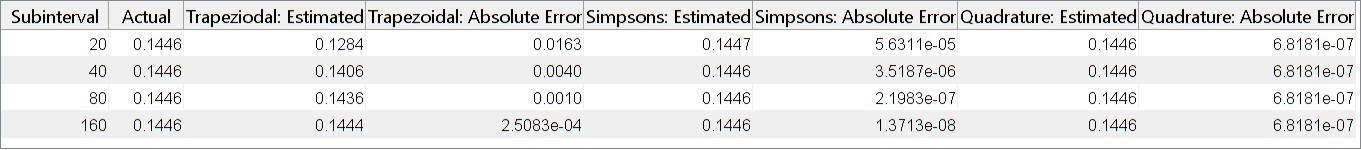
\includegraphics[width=1.1\linewidth]{table.jpg}
    \caption{Comparison Table}\label{fig:Comparison_Table}
\end{figure}

The adaptive quadrature does not have any integration subintervals. It is more used in the table to compare to the other integration techniques.

Out of the composite trapezoidal rule and composite Simpson's rule, the composite Simpson's rule faired much better as it has a smaller error degree than the composite trapezoidal rule $\mathcal{O}(h^{5})$ for the Simpson's rule versus $\mathcal{O}(h^{3})$ for the trapezoidal rule.

The adaptive quadrature was generally more accurate than the two composite rules, except for the 80 and 160 integration subinterval of the composite Simpson's rule. If the tolerance for the adaptive quadrature had been set at a much lower value than $10^{-4}$, then the adaptive quadrature would have a higher accuracy. However, setting a lower tolerance would be at the expense of computing time.

\pagebreak
\lstset{title={Homework 4: main.m}}
\begin{lstlisting}[language = Matlab]
%% Zack Humphries
% COMP 521
% HW4

% Use numerical integration to approximate the integral of a function f(x)
% over the interval x \in [a,b]
close all; clear all; clc;

a = 0;
b = 3.5;
n_list = [20 40 80 160];
length_n_list = length(n_list);
trapl_array = zeros(1,length_n_list);
simprl_array = zeros(1,length_n_list);

for n_index=1:length_n_list

    n = n_list(n_index);
    % Part 1
    % Apply the somposite trapezoidal rule to calculate the integral
    Itc = traprl(@Fx, a, b, n);
    fprintf("The result for the integral with n = %f using Trapezoidal is %.16f \n", n, Itc);
    
    
    % Part 2
    % Apply the somposite Simpson's Rule to calculate the integral
    Isc = simprl(@Fx, a, b, n);
    fprintf("The result for the integral with n = %f using Simpson's is %.16f \n", n, Isc);
    
        
    trapl_array(n_index) = Itc;
    simprl_array(n_index) = Isc;
end

% Part 3
% Apply adadptive quadrature to calculate the integral
tol = 1e-4;
[SRmat, Ias, err] = adapt(@Fx, a, b, tol);
x = SRmat(2,:);
fprintf("The result for the integral using Adaptive Simpson's is %.16f \n", Ias);

actual = 0.1446445197;

trapl_error = abs(actual - trapl_array);
simprl_error = abs(actual - simprl_array);
adapt_error = abs(actual-Ias);
actual_list = repmat(actual, 1, length_n_list);

adapt_list = repmat(Ias, 1, length_n_list);
adapt_error_list = repmat(adapt_error, 1, length_n_list);

var_names = ['Subinterval', "Actual", "Trapeziodal: Estimated", "Trapezoidal: Absolute Error", "Simpsons: Estimated", "Simpsons: Absolute Error", "Quadrature: Estimated", "Quadrature: Absolute Error"];

T = table(n_list.', actual_list.', trapl_array.', trapl_error.', simprl_array.', simprl_error.', adapt_list.', adapt_error_list.', VariableNames=var_names)
uitable('Data',T{:,:},'ColumnName',T.Properties.VariableNames,...
    'RowName',T.Properties.RowNames,'Units', 'Normalized', 'Position',[0, 0, 1, 1]);


function result = Fx(x)
    part1 = exp(-2*x);
    part2 = sin(2*pi*x);
    result = part1.*part2;
end
\end{lstlisting}



\end{document}